\clearpage % Rozdziały zaczynamy od nowej strony.
\section{Walidacja działania metody}

Do wygenerowania danych użyto informacji z TLE (Two Line Element) Międzynarodowej Stacji Kosmicznej z 19 grudnia 2022, pobranych ze strony archiwizującej informacje o satelitach CelesTrak \cite{Celestrak}:
\begin{verbatim}
1 25544U 98067A   22353.42711160  .00011227  00000-0  20403-3 0  9992
2 25544  51.6432 138.9346 0003592 174.7295 234.7524 15.50052736373915
\end{verbatim}

Format TLE nie zawiera informacji o elementach orbitalnych zdefiniowanych tak jak w rozdziale \ref{ch:wektory-stanu}. Zamiast półosi wielkiej podaje dodatkowe informacje takie jak średnia częstość kołowa, jej pierwszą i drugą pochodną, współczynnik ciśnienia promieniowania, anomalię średnią oraz informacje o obiekcie i orbicie \cite{TLE}.

Półoś wielką można wyznaczyć na podstawie częstości kołowej zgodnie ze wzorem:
\begin{equation}
a = \frac{\mu^{\frac{1}{3}}}{\left(\frac{2\pi}{24\cdot60\cdot60}n\right)^{\frac{2}{3}}}
\end{equation}
Gdzie: 
\begin{itemize}
\item n -- częstość kołowa [obr/dzień]
\item       $\mu$ -- $GM$ standardowy parametr grawitacyjny dla Ziemi
\end{itemize}

Na podstawie danych TLE uzyskano klasyczne elementy orbitalne. Następnie wygenerowano trzy zestawy danych obserwacyjnych i wykonano 5 porównań:
\begin{itemize}
    \item trzy obserwacje w pobliżu górowania, o niewielkich różnicach czasu między obserwacjami 
    \item trzy obserwacje dokonane podczas wschodu, górowania i zachodu obserwowanego obiektu
    \item powyższe dwa przypadki z symulowanym błędem pomiaru
    \item sytuacja hipotetyczna - obserwacje równomiernie oddzielone na całej orbicie
    \item obserwacje dokonane w symulatorze nocnego nieba Stellarium
\end{itemize}

\subsection{Wspólne stałe}
Podczas wszystkich porównań przyjęto następujące wspólne stale:

        \begin{align*}
             \phi &= 51\degree 23'15.49" \\
             H &= 153 m \\
             R_{E} &= 6378 km \\
             f &= 0.003353 \\
             \mu &= 3,986004418 \cdot 10^{14} \frac{m^3}{s^2}
        \end{align*}
    Gdzie:
        \begin{itemize}
            \item  $ \phi$  -- szerokość geograficzna obserwatora 
            \item $H$ -- wysokość nad poziomem morza obserwatora
            \item       $ R_{E}$ -- promień Ziemi  
            \item        $f$ -- spłaszczenie Ziemi 
            \item $\theta$ -- lokalny czas gwiazdowy obserwacji
        \end{itemize}
        
Współrzędne kartezjańskie obserwatora dla każdej obserwacji wyznaczono ze wzoru:

            \begin{center}
            \begin{equation}
              \begin{split}
              \mathbf{R} & =\left[ \cfrac{R_e}{\sqrt{1-(2f-f^2)sin^2\phi}} + H\right]\cdot \cos{\phi}(\cos{{\theta}\hat{I}+\sin{\theta}\hat{J}}) \\
            &+  \left[ \cfrac{R_e(1-f)^2}{\sqrt{1-(2f-f^2)sin^2\phi}} + H\right] \cdot \sin{\phi} 
            \end{split}
            \end{equation}
        \end{center}



\FloatBarrier
\subsection{Obserwacja w pobliżu górowania}
\label{sub:Krotki}
      \subsubsection{Dane obserwacyjne}

    Czas obserwacji odpowiada zmianie anomalii o kąt 10\degree: 
        \begin{align*}
            t_{1} &= 0 s \\
            t_{2} &= 77 s  \\
            t_{3} &= 154 s
        \end{align*}    
        
    Czas gwiazdowy obserwacji: 
        \begin{align*}
            \theta_1 &= 301.7692\degree \\
            \theta_2 &= 302.0933\degree  \\
            \theta_3 &= 302.4175\degree
        \end{align*}

    Wykorzystane pozycje [km]: 
   
            \begin{center}
              $\begin{bmatrix}
                R_{1x} & R_{1y} & R_{1z} \\
                R_{2x} & R_{2y} & R_{2z} \\
                R_{3x} & R_{3y} & R_{3z} 
            \end{bmatrix}
            =
            \begin{bmatrix}
                338 & -5050 & 4530 \\
                843 & -5216 & 4269 \\
                1342 & -5342 & 3975
            \end{bmatrix}    $
        \end{center}

    \subsubsection{Wyniki}
    
    Wszystkie błędy są mniejsze niż 1e-06. Jest to zgodne z oczekiwaniami, ponieważ model obserwacyjny i metoda wyznaczania korzystają z idealnego modelu keplerowskiego.

    \begin{table}[!ht]  \centering
    \caption{Krótki czas między obserwacjami - porównanie wyników}
    \label{tab:Krotki-table}
    \begin{tabular} {| l | r | r | r |} \hline
        Parametr 1          & Wartość referencyjna  & Wartość wyznaczona  & Błąd \\ \hline\hline
        Moduł położenia w 2 pozycji     & 6793 km    & 6793 km        & 1e-09 km\\ \hline
        Moduł prędkości w 2 pozycji     & 7.7 km/s     & 7.7 km/s     & 5e-11 km/s\\ \hline
        Mimośród                        & 3.6e-04       & 3.6e-04      & 2e-12 \\ \hline
        Półoś wielka                    & 6794 km    & 6794 km        & 2e-08 \\ \hline
        Inklinacja                      & 51.64\degree & 51.64\degree & 3e-11\degree \\ \hline
        Rektascensja węzła wstępującego & 138.9\degree & 138.9\degree & 4e-11 \degree \\ \hline
        Argument perycentrum            & 174.7\degree & 174.7\degree  & 4e-07 \\ \hline
        Anomalia prawdziwa              & 312\degree   & 312\degree   & 4e-07 \\ \hline
    \end{tabular}
    \end{table}

    \begin{figure}[h]
    \centering
    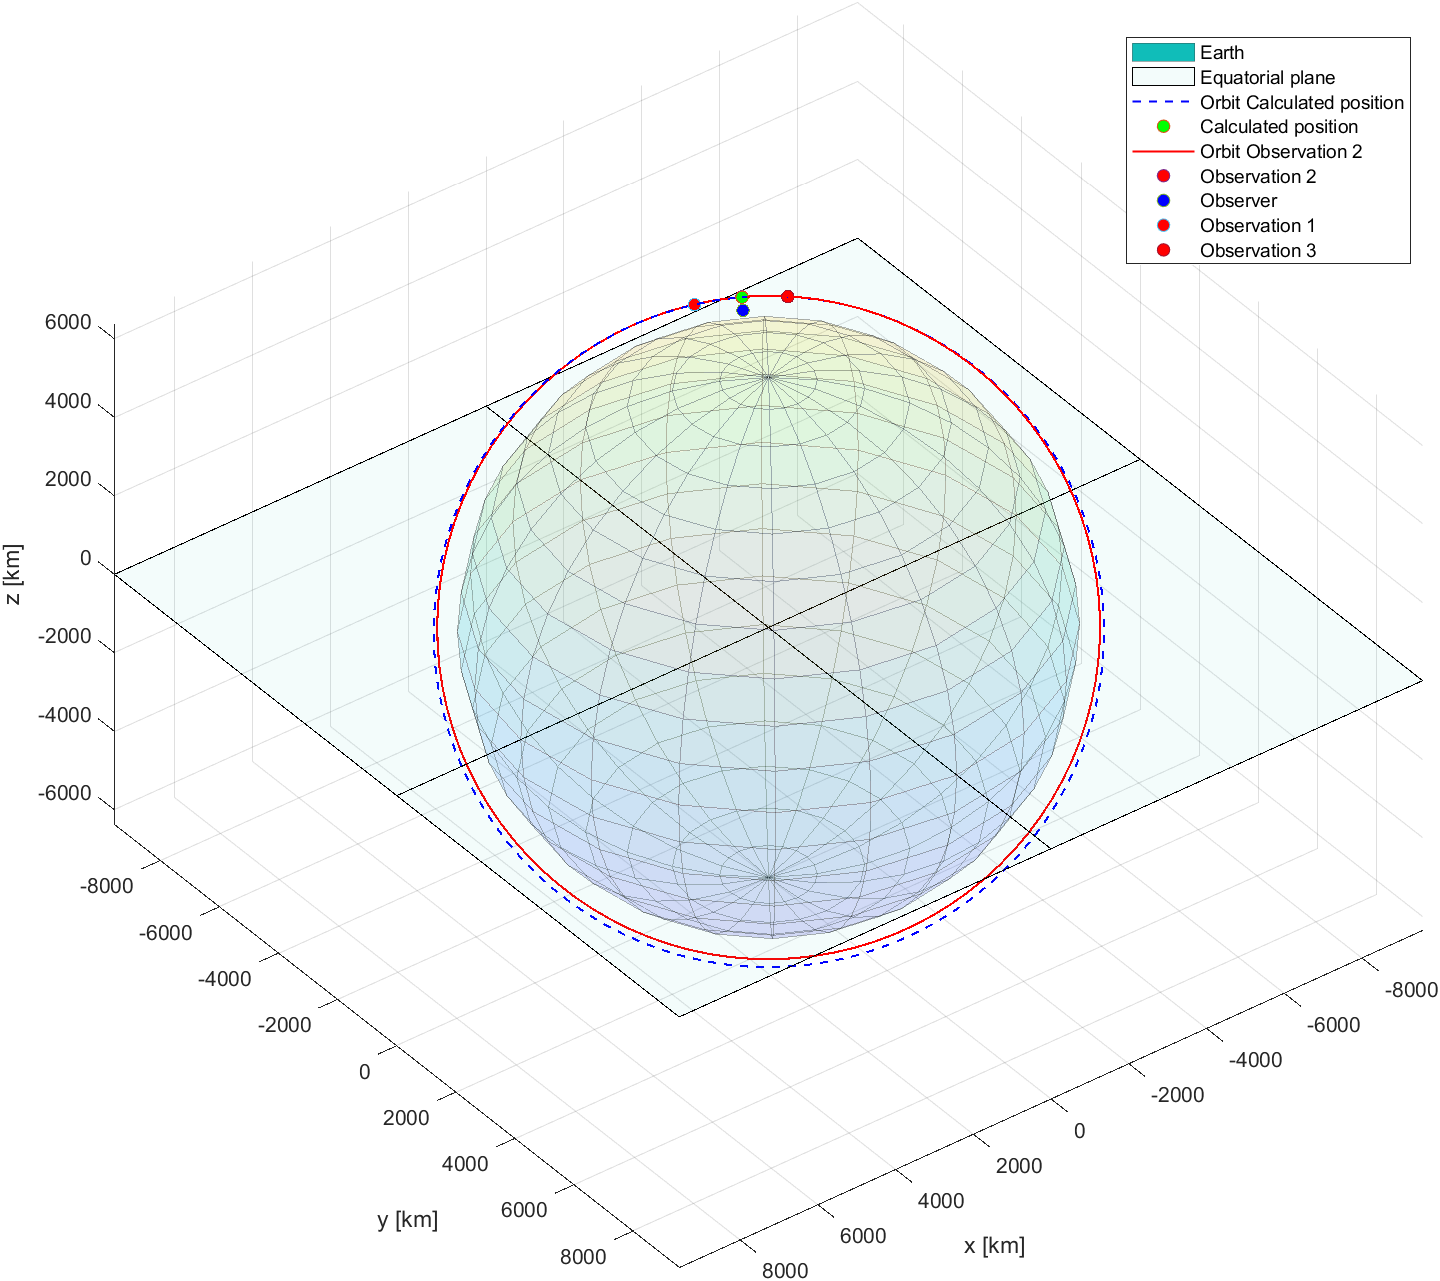
\includegraphics[width=\textwidth]{tex/img/StellariumFigure.png}
    \caption{Krótki czas między obserwacjami - wizualizacja}
    \label{fig:Krotki-1}
    \end{figure}
    
    \begin{figure}[h]
    \centering
    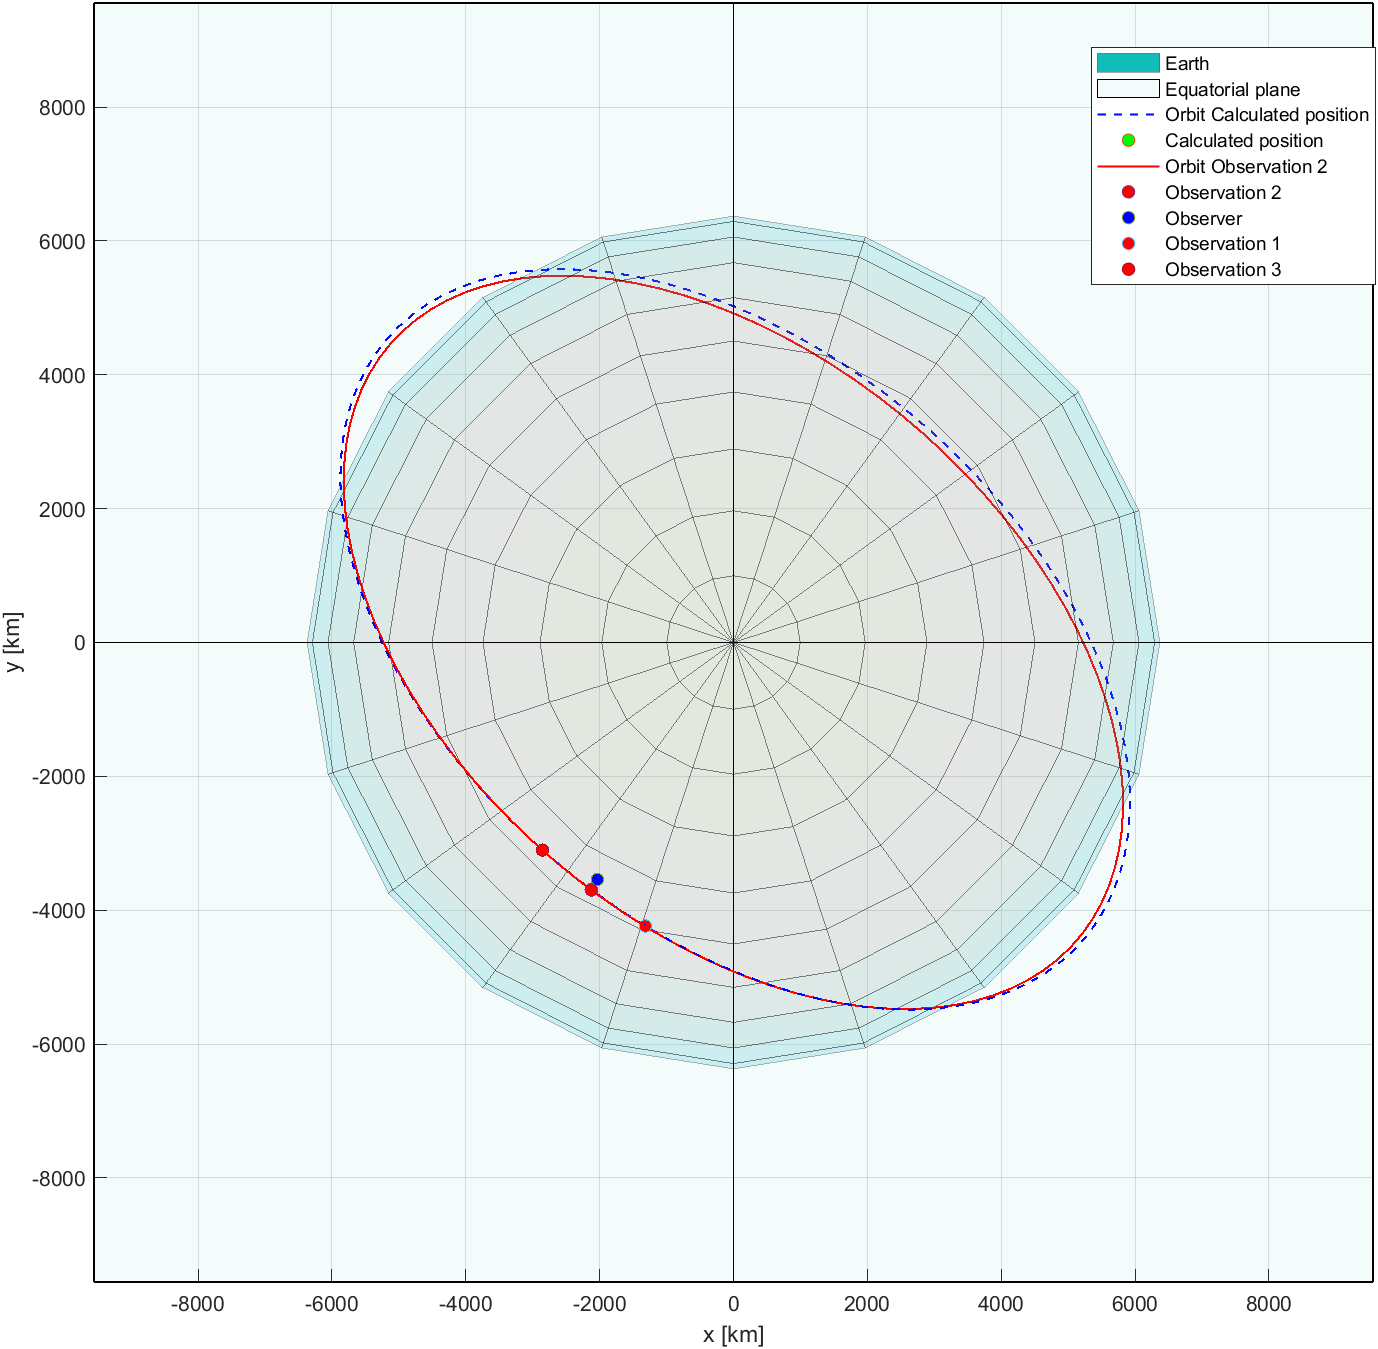
\includegraphics[width=\textwidth]{tex/img/StellariumFigure_rownikowa.png}
    \caption{Krótki czas między obserwacjami - rzut na płaszczyznę równikową}
    \label{fig:Krotki-2}
    \end{figure}


\FloatBarrier
\subsection{Obserwacja podczas pełnego przelotu}
\label{sub:Pelny}
       \subsubsection{Dane obserwacyjne}

    Czas obserwacji odpowiada zmianie anomalii o kąt 30\degree: 
        \begin{align*}
            t_{1} &= 0 s \\
            t_{2} &= 309 s  \\
            t_{3} &= 619 s
        \end{align*}    
        
    Czas gwiazdowy obserwacji: 
        \begin{align*}
            \theta_1 &= 300.7965\degree \\
            \theta_2 &= 302.0933\degree  \\
            \theta_3 &= 303.3900\degree
        \end{align*}

    Wykorzystane pozycje [km]: 
   
            \begin{center}
              $\begin{bmatrix}
                R_{1x} & R_{1y} & R_{1z} \\
                R_{2x} & R_{2y} & R_{2z} \\
                R_{3x} & R_{3y} & R_{3z} 
            \end{bmatrix}
            =
            \begin{bmatrix}
                -1177 & -4328 & 5101 \\
                843 & -5216 & 4269 \\
                2762 & -5474 & 2922
            \end{bmatrix}    $
        \end{center}

    \subsubsection{Wyniki}
    
    Wszystkie błędy są mniejsze niż 1e-06, podobnie jak dla obserwacji o krótkich odstępach między pomiarami.

    \begin{table}[!h] \centering
    \caption{Obserwacje rozproszone - porównanie wyników}
    \label{tab:Dlugi-table}
    \begin{tabular} {| l | r | r | r |} \hline
        Parametr 1          & Wartość referencyjna  & Wartość wyznaczona  & Błąd \\ \hline\hline
        Moduł położenia w 2 pozycji     & 6793 km    & 6793 km        & 1e-09 km\\ \hline
        Moduł prędkości w 2 pozycji     & 7.7 km/s     & 7.7 km/s     & 5e-11 km/s\\ \hline
        Mimośród                        & 3.6e-04       & 3.6e-04      & 1e-11 \\ \hline
        Półoś wielka                    & 6794 km    & 6794 km        & 9e-08 \\ \hline
        Inklinacja                      & 51.64\degree & 51.64\degree & 3e-11\degree \\ \hline
        Rektascensja węzła wstępującego & 138.9\degree & 138.9\degree & 7e-13 \degree \\ \hline
        Argument perycentrum            & 174.7\degree & 174.7\degree  & 1e-06 \\ \hline
        Anomalia prawdziwa              & 312\degree   & 312\degree   & 1e-06 \\ \hline
    \end{tabular}
    \end{table}

    \begin{figure}[h]
    \centering
    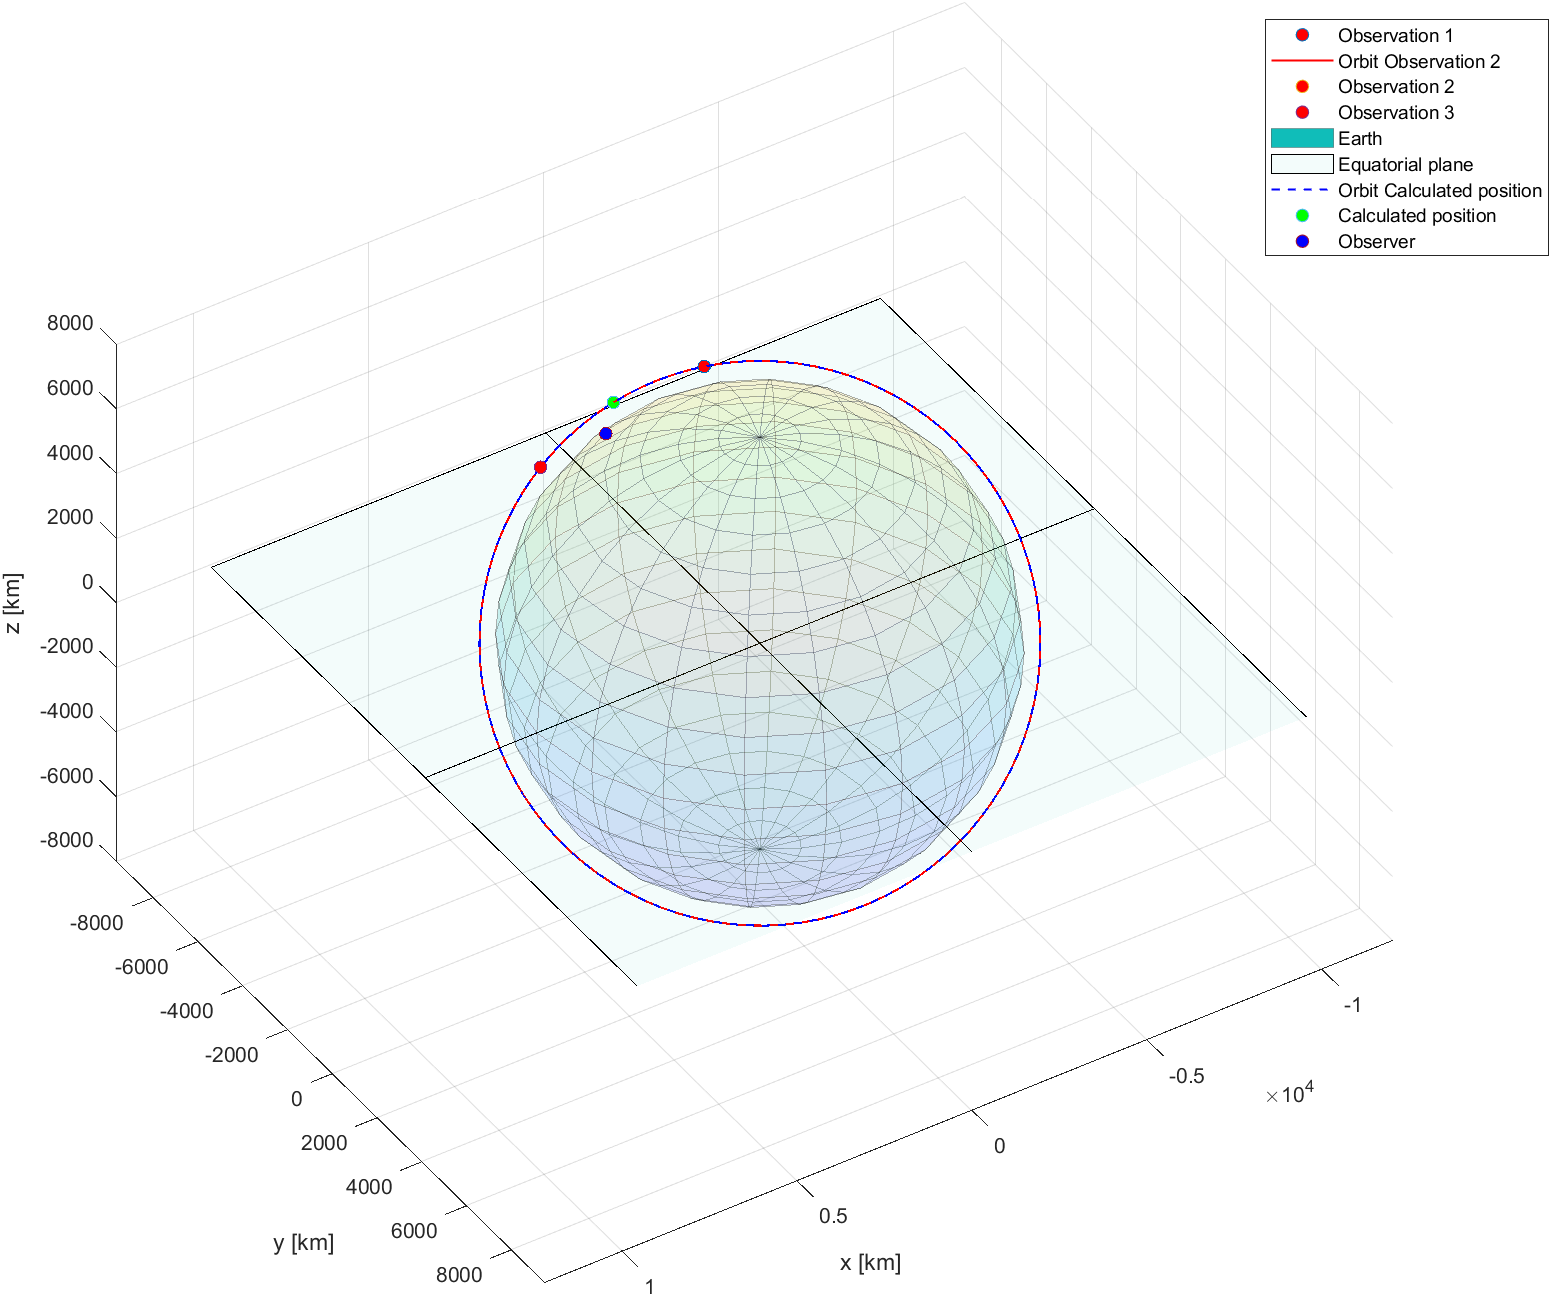
\includegraphics[width=\textwidth]{tex/img/anomaly15.png}
    \caption{Obserwacje rozproszone - wizualizacja}
    \label{fig:Dlugi-1}
    \end{figure}
    
    \begin{figure}[h]
    \centering
    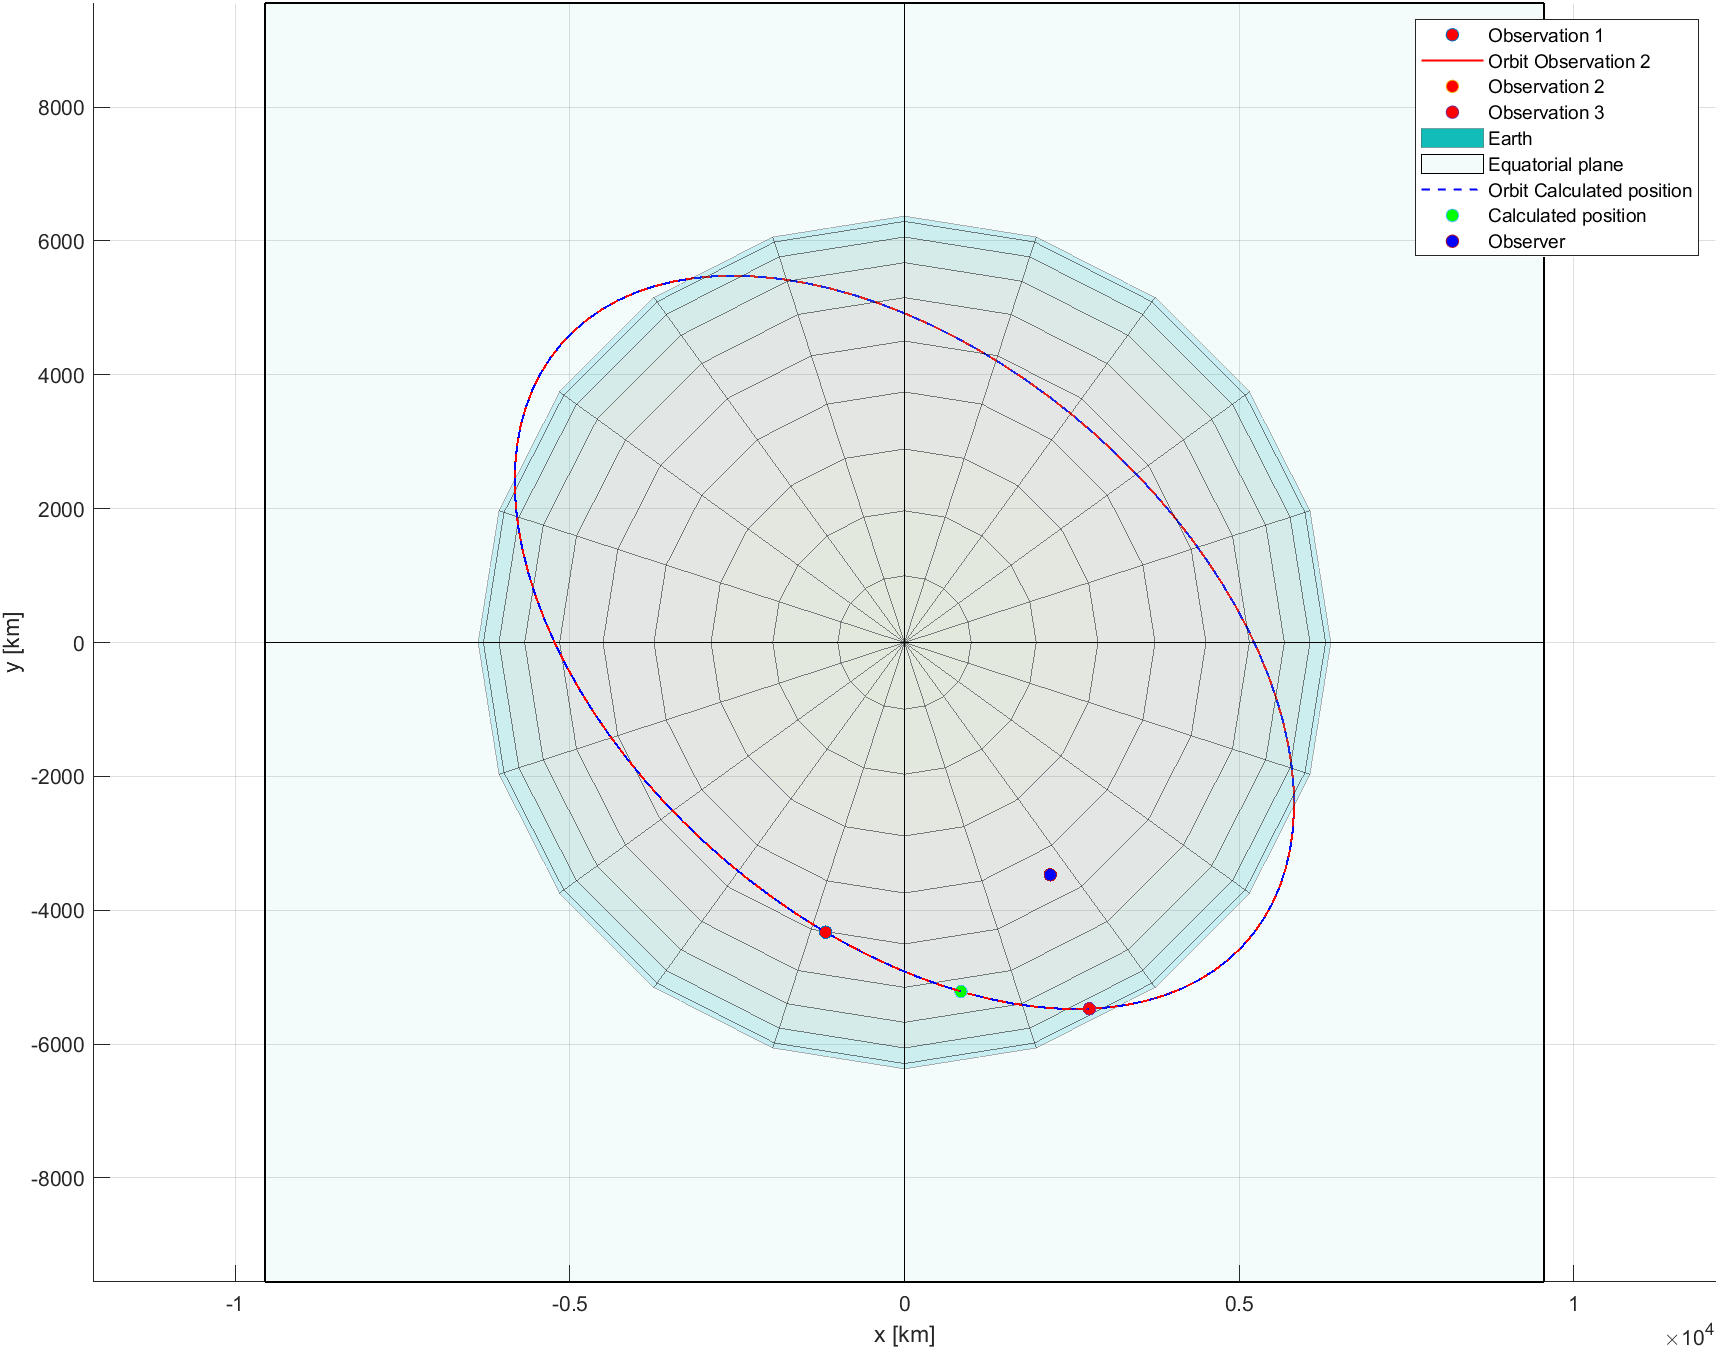
\includegraphics[width=\textwidth]{tex/img/anomaly15_rownikowa.png}
    \caption{Obserwacje rozproszone - rzut na płaszczyznę równikową}
    \label{fig:Dlugi-2}
    \end{figure}



\FloatBarrier
\subsection{Obserwacje zakłócone}

Wyniki uzyskane w podrozdziałach \ref{sub:Krotki} i \ref{sub:Pelny} sugerują, że rozkładanie obserwacji w czasie może nie mieć wpływu na wyniki, ponieważ nawet dla krótkich obserwacji błędy praktycznie nie istnieją. Jest to jednak spowodowane tym, że dane obserwacyjne są generowane w sposób idealny na podstawie idealnego modelu. Poniżej przedstawiono wyniki dla pomiarów nieidealnych.

     \subsubsection{Dane obserwacyjne}
    Takie jak w rozdziałach \ref{sub:Krotki} i \ref{sub:Pelny}. Wersory kierunkowe zaszumiono dodając do każdej współrzędnej losowe liczby z przedziału [0; 0,002] i ponowownie normalizując.
    
    \subsubsection{Wyniki}
    Wyznaczone orbity zostały jakościowo porównane na wykresie \ref{fig:szum_side_by_side}. Zgodnie z oczekiwaniami przeprowadzenie pomiarów z większymi interwałami czasowymi pozwala na wyznaczenie orbity mimo nieidealnych danych.

\begin{figure}%
    \centering
    \subfloat[\centering Krótki czas między obserwacjami]{{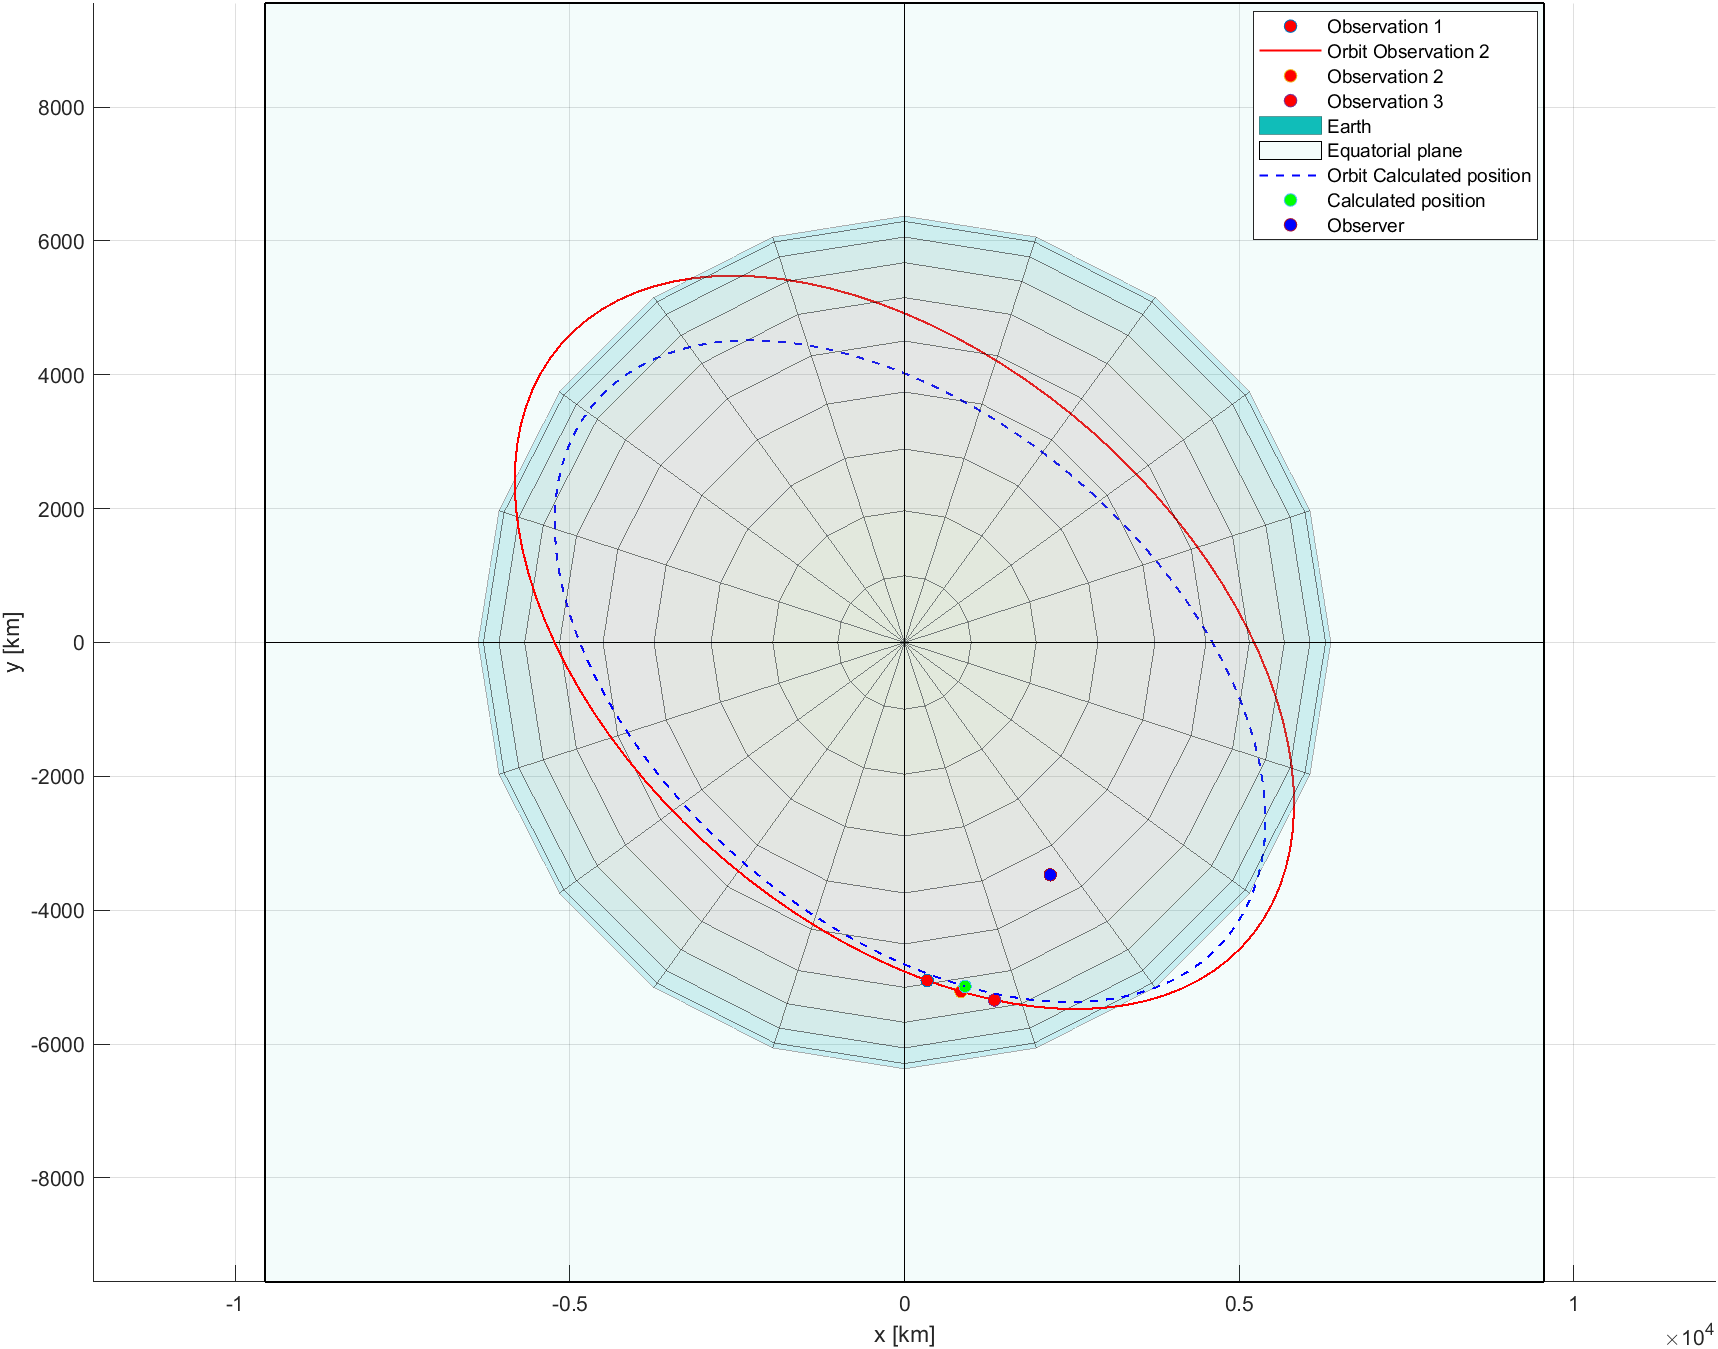
\includegraphics[width=13cm]{tex/img/szum5_rownik.png} }}%
    \qquad
    \subfloat[\centering Obserwacje rozproszone w czasie]{{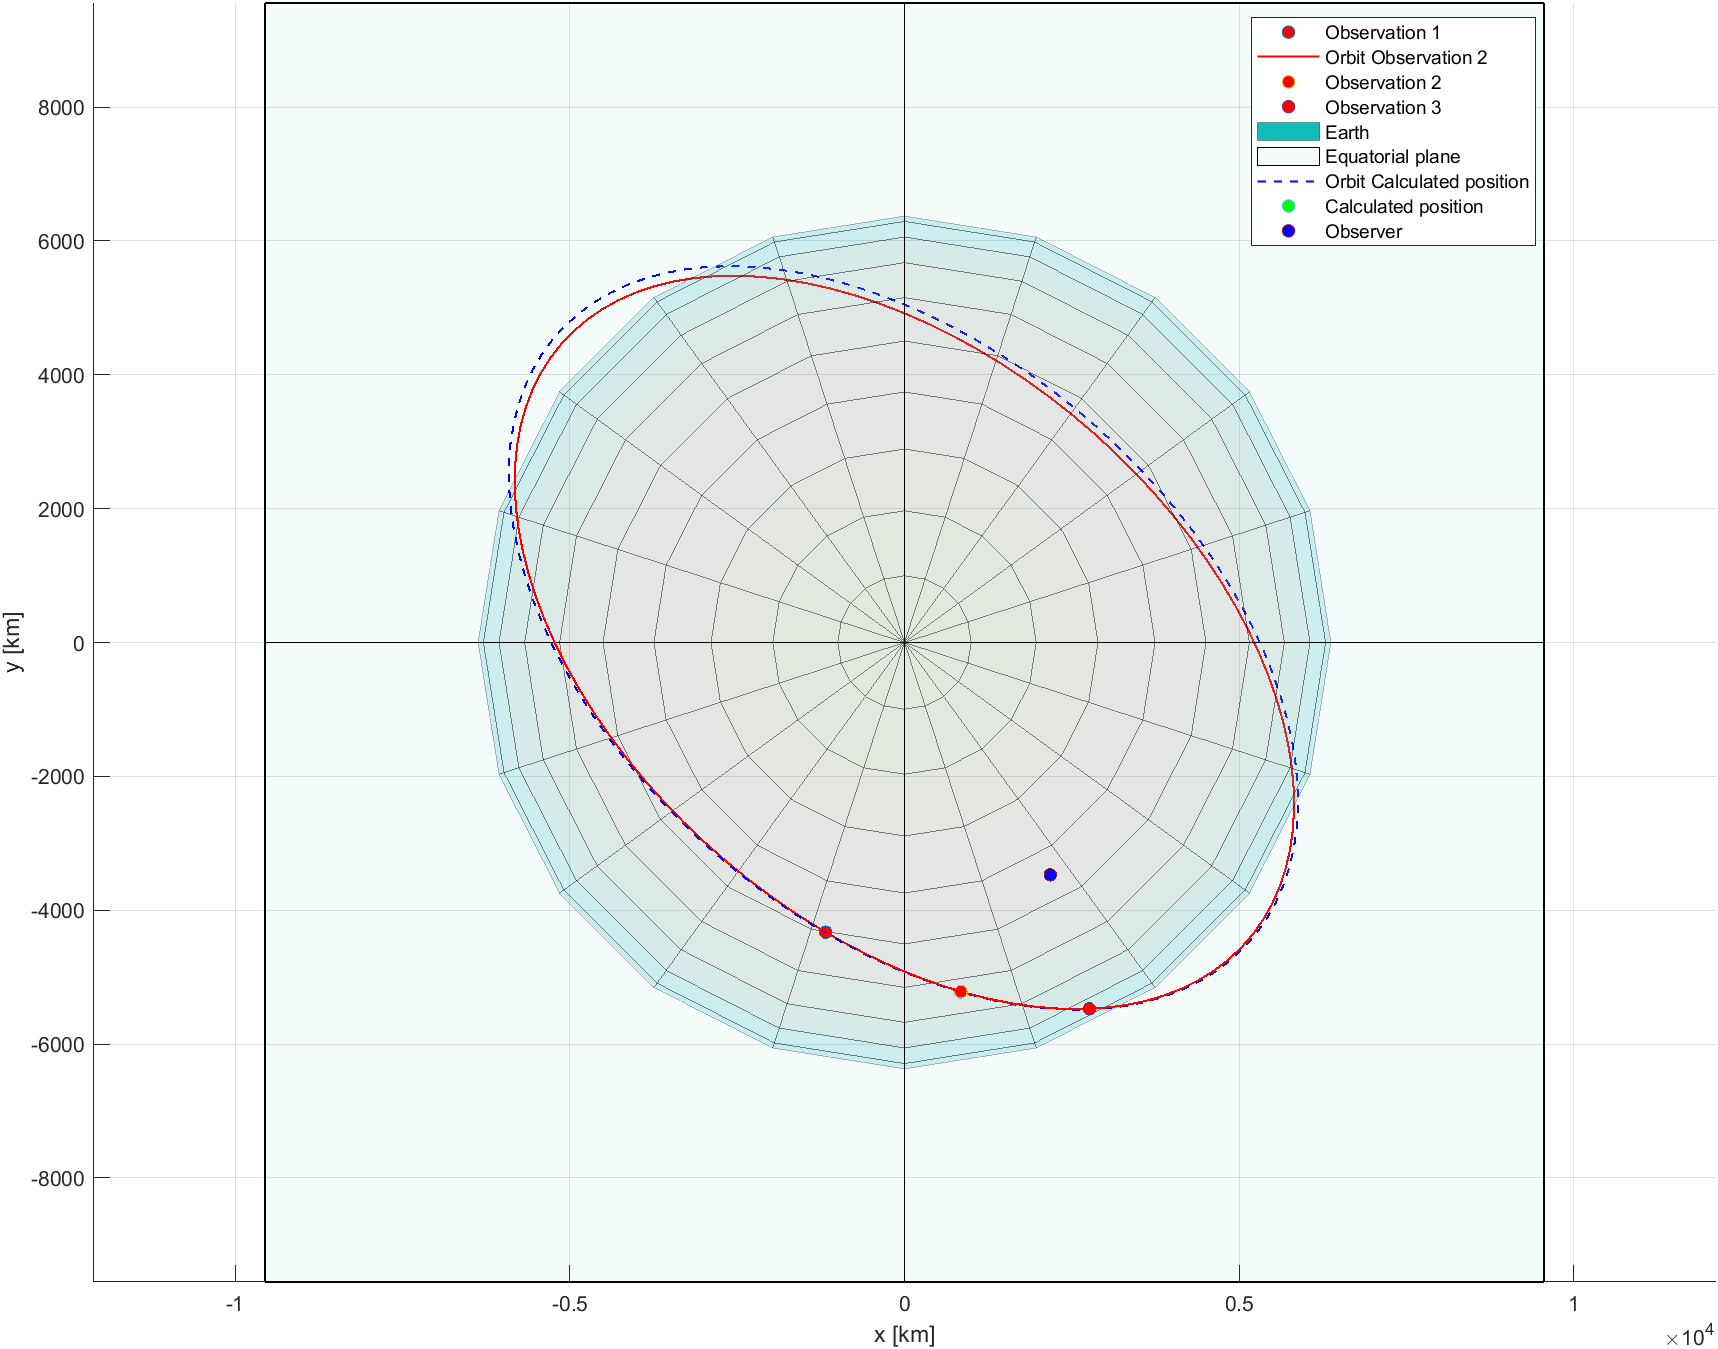
\includegraphics[width=13cm]{tex/img/szum15_rownik.png} }}%
    \caption{Porównanie wpływu dodanego błędu do wersora kierunkowego obserwacji na określoną orbitę w dla dwóch częstości dokonywania pomiarów}%
    \label{fig:szum_side_by_side}%
\end{figure}

\FloatBarrier
\subsection{Obserwacja hipotetyczna}

     \subsubsection{Dane obserwacyjne}

    Czas obserwacji odpowiada zmianie anomalii o kąt 162:\degree: 
        \begin{align*}
            t_{1} &= 0 s \\
            t_{2} &= 1269 s  \\
            t_{3} &= 2538 s
        \end{align*}    
        
    Czas gwiazdowy obserwacji: 
        \begin{align*}
            \theta_1 &= 296.7743\degree \\
            \theta_2 &= 302.0933\degree  \\
            \theta_3 &= 307.4090\degree
        \end{align*}

    Wykorzystane pozycje [km]: 
   
            \begin{center}
              $\begin{bmatrix}
                R_{1x} & R_{1y} & R_{1z} \\
                R_{2x} & R_{2y} & R_{2z} \\
                R_{3x} & R_{3y} & R_{3z} 
            \end{bmatrix}
            =
            \begin{bmatrix}
                -5590 & 934 & 3750 \\
                843 & -5216 & 4269 \\
                5821 & -2385 & -2560
            \end{bmatrix}    $
        \end{center}

    
    \subsubsection{Wyniki}
    Ponieważ wyprowadzenie metody Gaussa wykorzystuje założenie, że czas między pomiarami jest niewielki względem okresu orbity \cite{Curtis2013}, to jest ona nieskuteczna dla długich obserwacji. Zastosowanie poprawki iteracyjnej pozwala na powiększenie zakresu stosowalności, ale ostatecznie i ona zawodzi, gdy metoda podstawowa przestaje generować wystarczająco zbliżone wyniki. Dla przeprowadzonych symulacji maksymalna zmiana anomalii prawdziwej, dla których metoda zwracała poprawne wyniki, wynosiła 160\degree. 

    \begin{figure}[h]
    \centering
    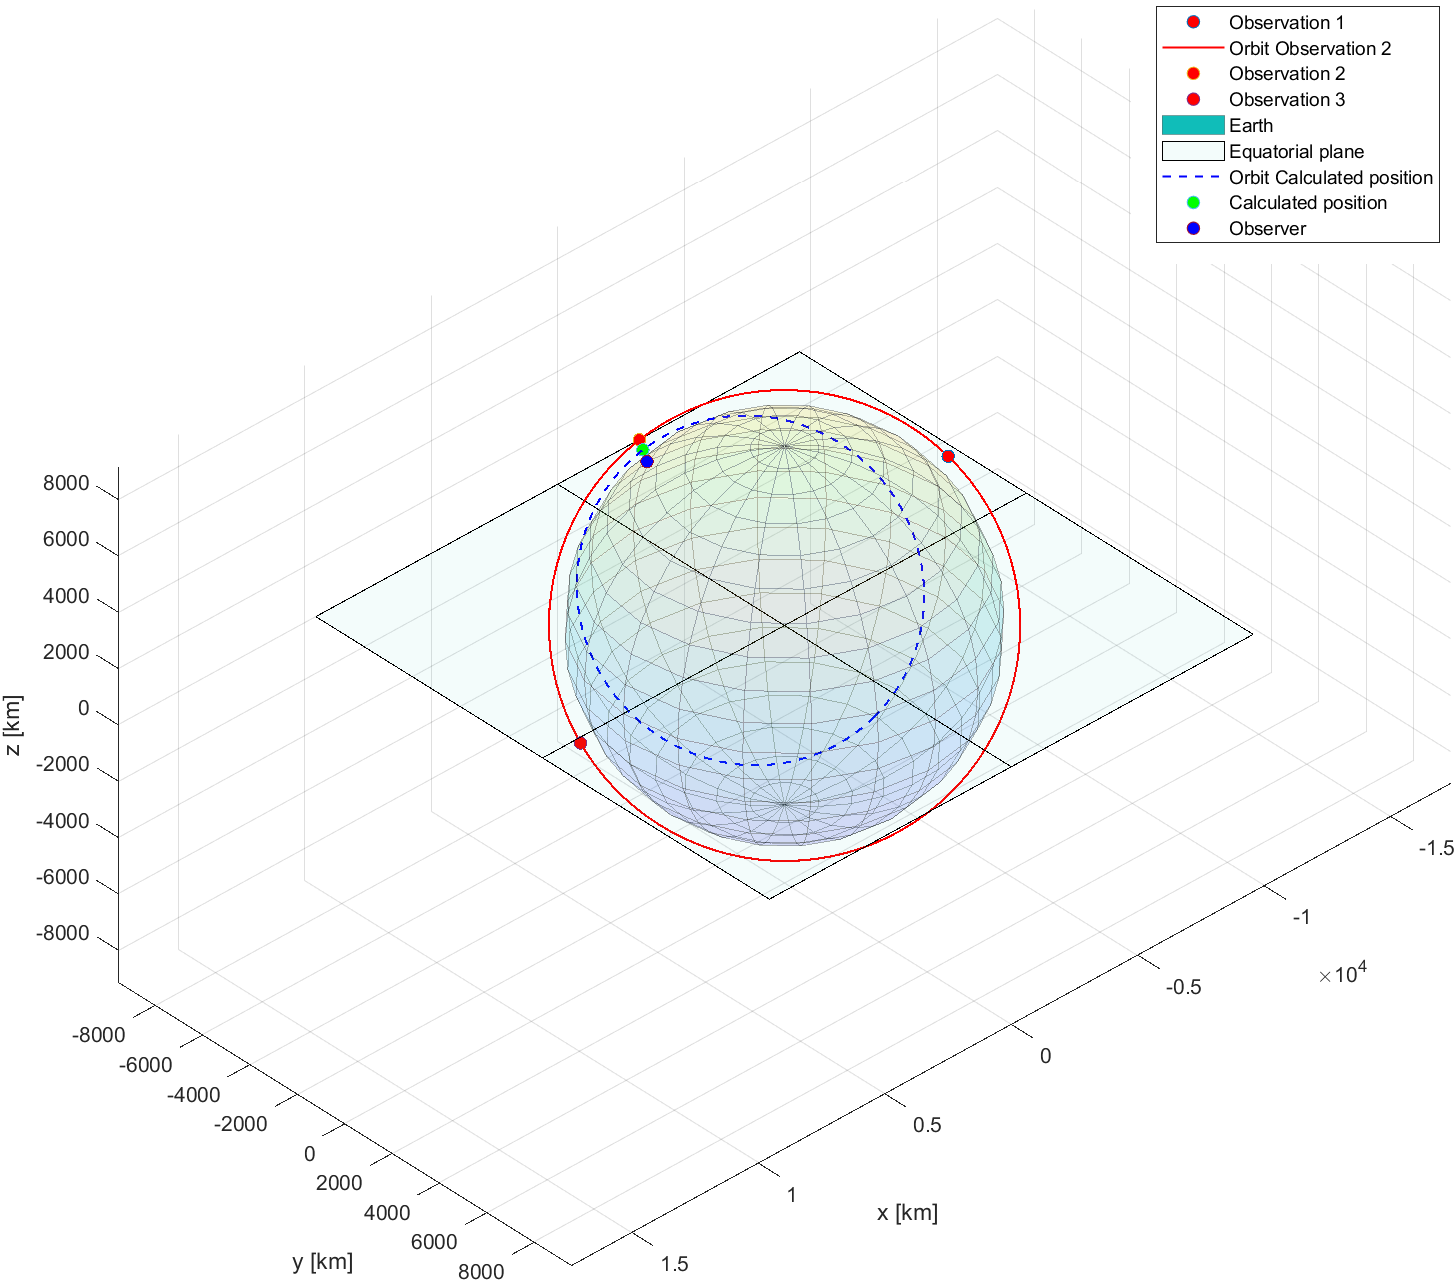
\includegraphics[width=\textwidth]{tex/img/anomaly82.png}
    \caption{Obserwacje hipotetyczne - wizualizacja}
    \label{fig:hipotetyczne-1}
    \end{figure}
    
    \begin{figure}[h]
    \centering
    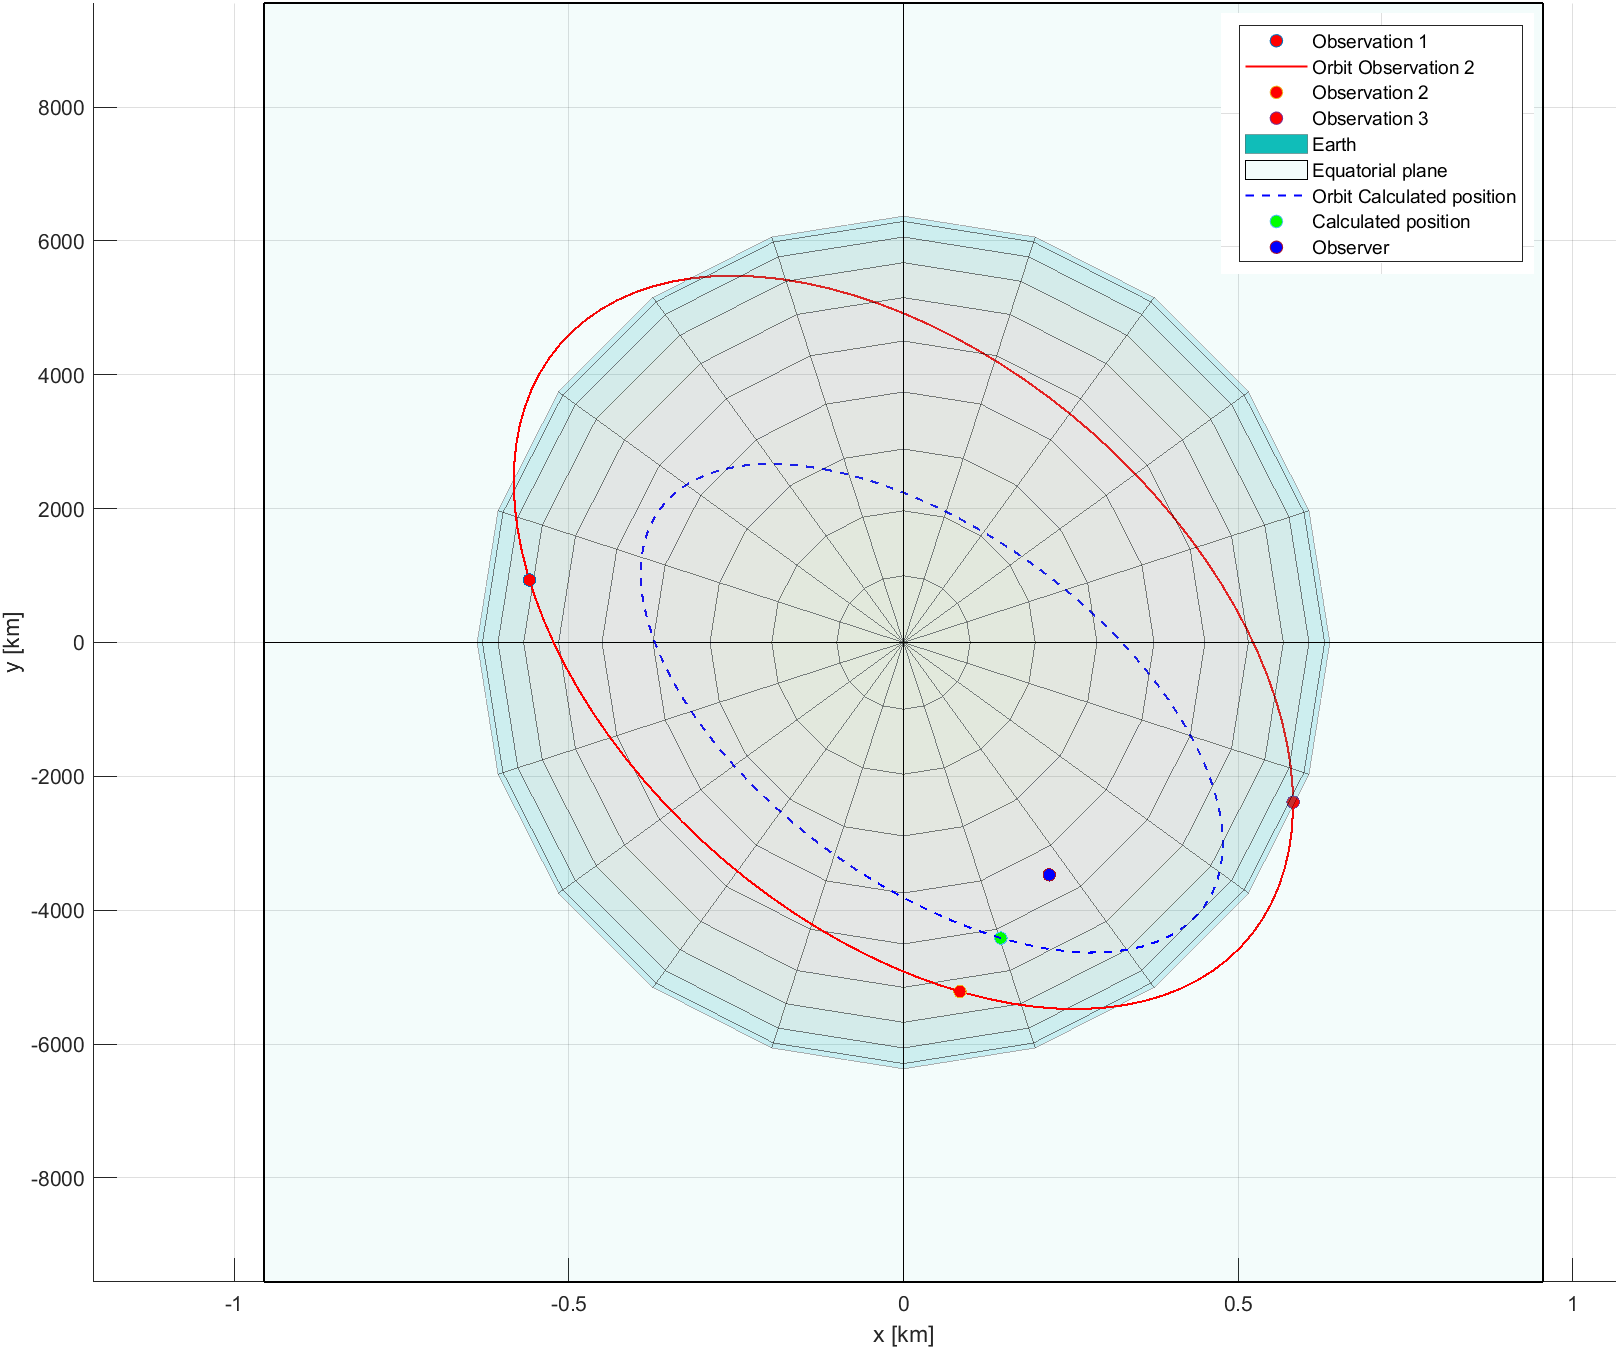
\includegraphics[width=\textwidth]{tex/img/anomaly82_rownikowa.png}
    \caption{Obserwacje hipotetyczne - rzut na płaszczyznę równikową}
    \label{fig:hipotetyczne-2}
    \end{figure}


\FloatBarrier
\subsection{Obserwacja rzeczywista}
 Do obserwacji wykorzystano program Stellarium. Interfejs aplikacji pokazuje Rys. \ref{fig:stellarium-interfejs}. Obserwatora umieszczono na współrzędnych 51\degree 23' 15" N, 18\degree 34' 10" E. Zaobserwowano przelot, który odbył się 19 grudnia 2022 między godziną 8:52 i 8:57 UTC. Czas wybrano z uwagi na zgodność daty z TLE i długi okres widoczności.
    \begin{figure}
    \centering
    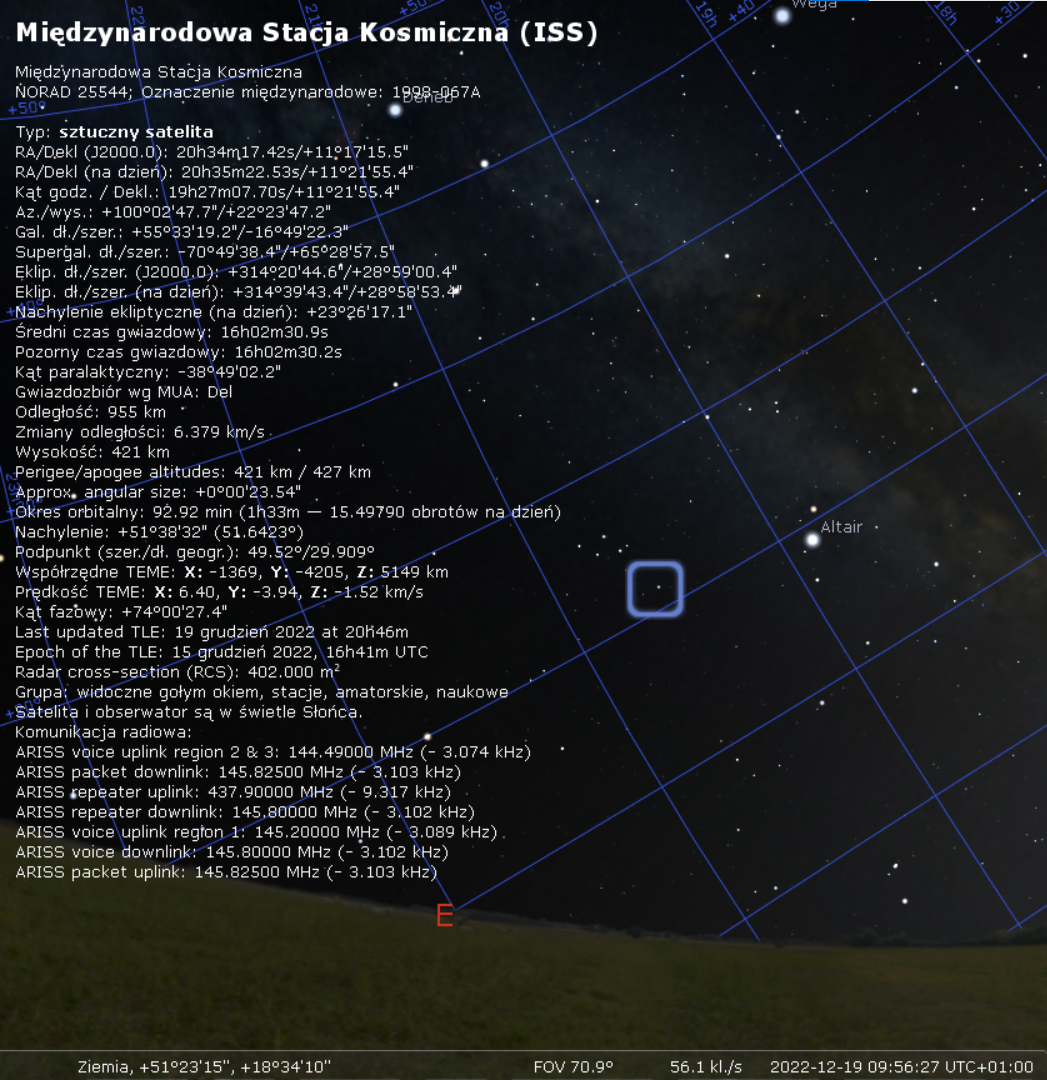
\includegraphics[width=\textwidth]{tex/img/ISSStellarium.png}
    \caption{Interfejs symulatora nocnego nieba Stellarium wykorzystanego do dokonania obserwacji}
    \label{fig:stellarium-interfejs}
    \end{figure}

    \subsubsection{Dane obserwacyjne}

    Czas obserwacji: 
        \begin{align*}
            t_1 &= 52'24" \\
            t_2 &= 54'26"  \\
            t_3 &= 56"35'
        \end{align*}
        
    Czas gwiazdowy obserwacji: 
        \begin{align*}
            \theta_1 &= 15\degree 28'27.1" \\
            \theta_2 &= 16\degree 00'29.8"  \\
            \theta_3 &= 16\degree 02'39.0"
        \end{align*}

    Wykorzystane pozycje [km]: 
   
            \begin{center}
              $\begin{bmatrix}
                R_{1x} & R_{1y} & R_{1z} \\
                R_{2x} & R_{2y} & R_{2z} \\
                R_{3x} & R_{3y} & R_{3z} 
            \end{bmatrix}
            =
            \begin{bmatrix}
                -2854 & -3102 & 5302 \\
                -2127 & -3692 & 5284 \\
                -1317 & -4237 & 5136
            \end{bmatrix}    $
        \end{center}

    \subsubsection{Wyniki}
    
    Pozycja wyznaczona przez program Stellarium pochodzi z bardziej zaawansowanego modelu, niż ten wykorzystywany do aproksymacji, co tłumaczy brak zgodności wyników. Mimo tego orbita została wyznaczone w przybliżeniu poprawnie, chociaż jest ona bardziej ekscentryczna. 

    \begin{table}[!h]  \centering
    \caption{Obserwacja rzeczywista - porównanie wyników}
    \label{tab:Stellarium-table}
    \begin{tabular} {| l | r | r | r |} \hline
        Parametr 1          & Wartość referencyjna  & Wartość wyznaczona  & Błąd \\ \hline\hline
        Moduł położenia w 2 pozycji     & 6788 km   & 6789         & 0.77 km\\ \hline
        Moduł prędkości w 2 pozycji     & 7.7 km/s     & 7.7 km/s     & 0.04 km/s\\ \hline
        Mimośród                        & 0.0004       & 0.0123       & 0.0119 \\ \hline
        Półoś wielka                    & 6794 km    & 6873 km        & 78 km \\ \hline
        Inklinacja                      & 51.64\degree & 51.63\degree & -0.018\degree \\ \hline
        Rektascensja węzła wstępującego & 138.9\degree & 139.2\degree & 0.23 \degree \\ \hline
        Argument perycentrum            & 174.7\degree & 97.6\degree  & -76.9 \\ \hline
        Anomalia prawdziwa              & 282\degree   & 356\degree   & 74 \\ \hline
    \end{tabular}
    \end{table}

    \begin{figure}[h]
    \centering
    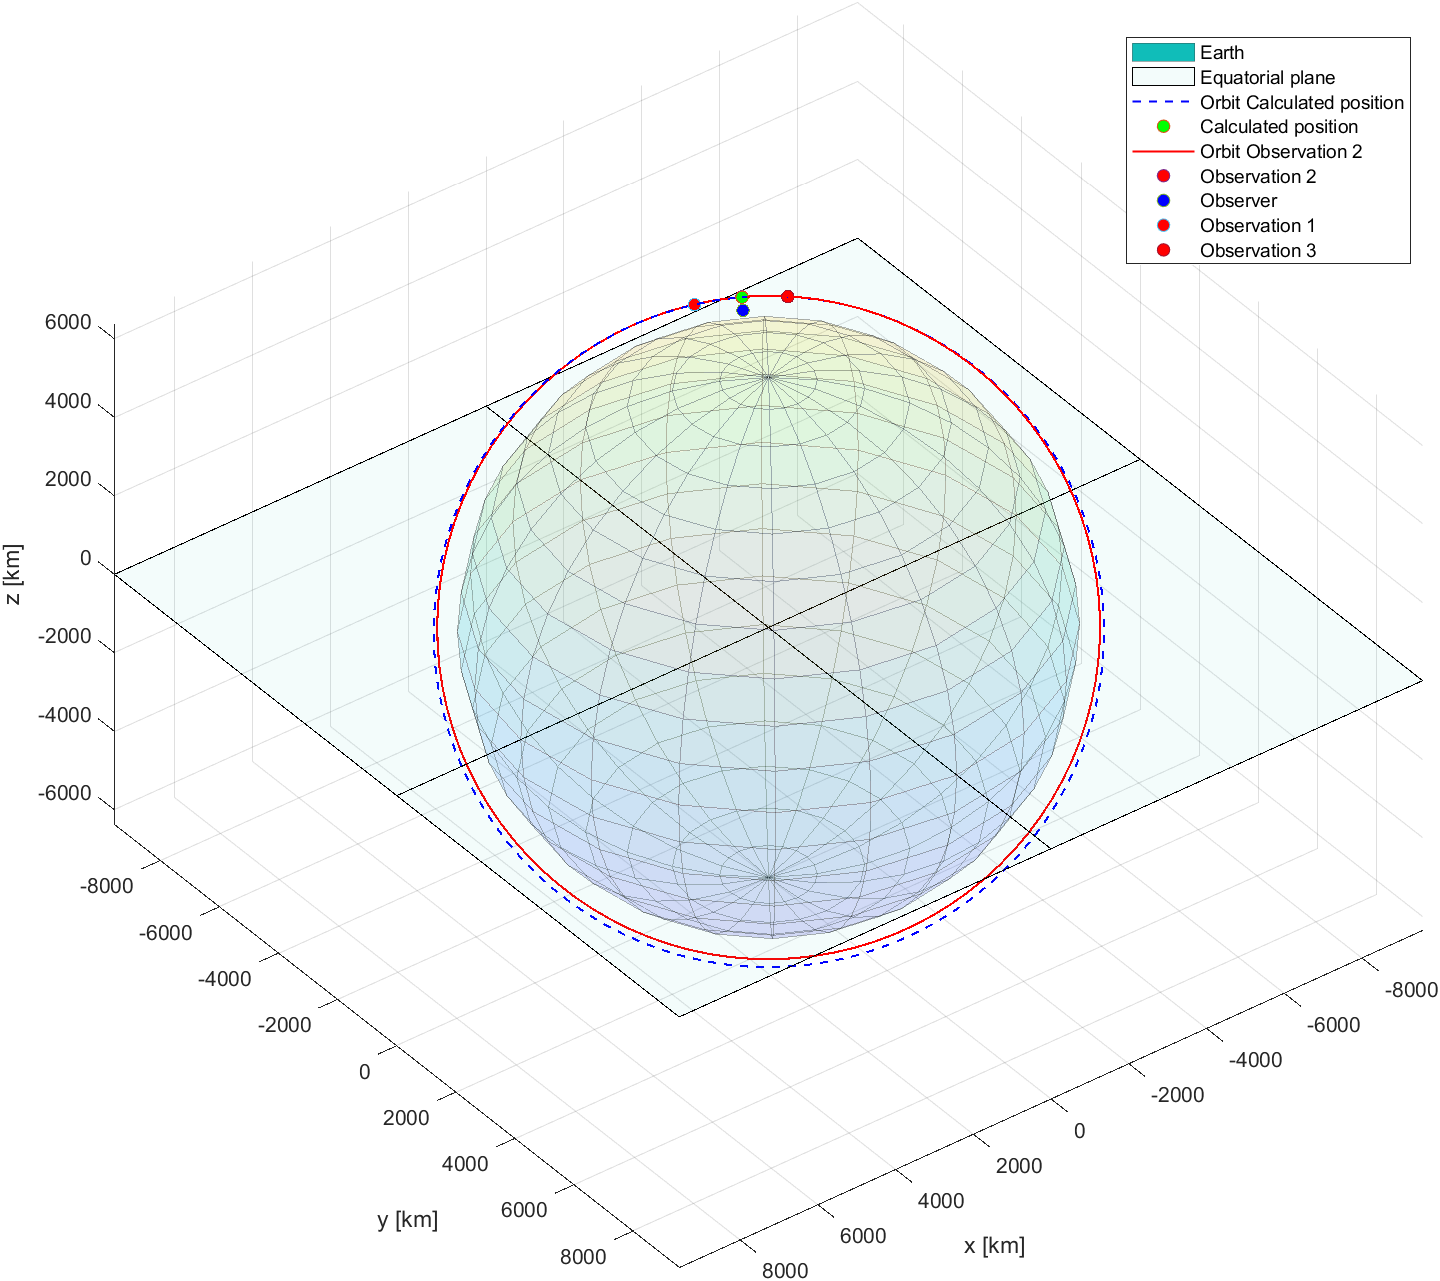
\includegraphics[width=\textwidth]{tex/img/StellariumFigure.png}
    \caption{Obserwacja na podstawie symulatora nieba}
    \label{fig:Stellarium-1}
    \end{figure}
    
    \begin{figure}[h]
    \centering
    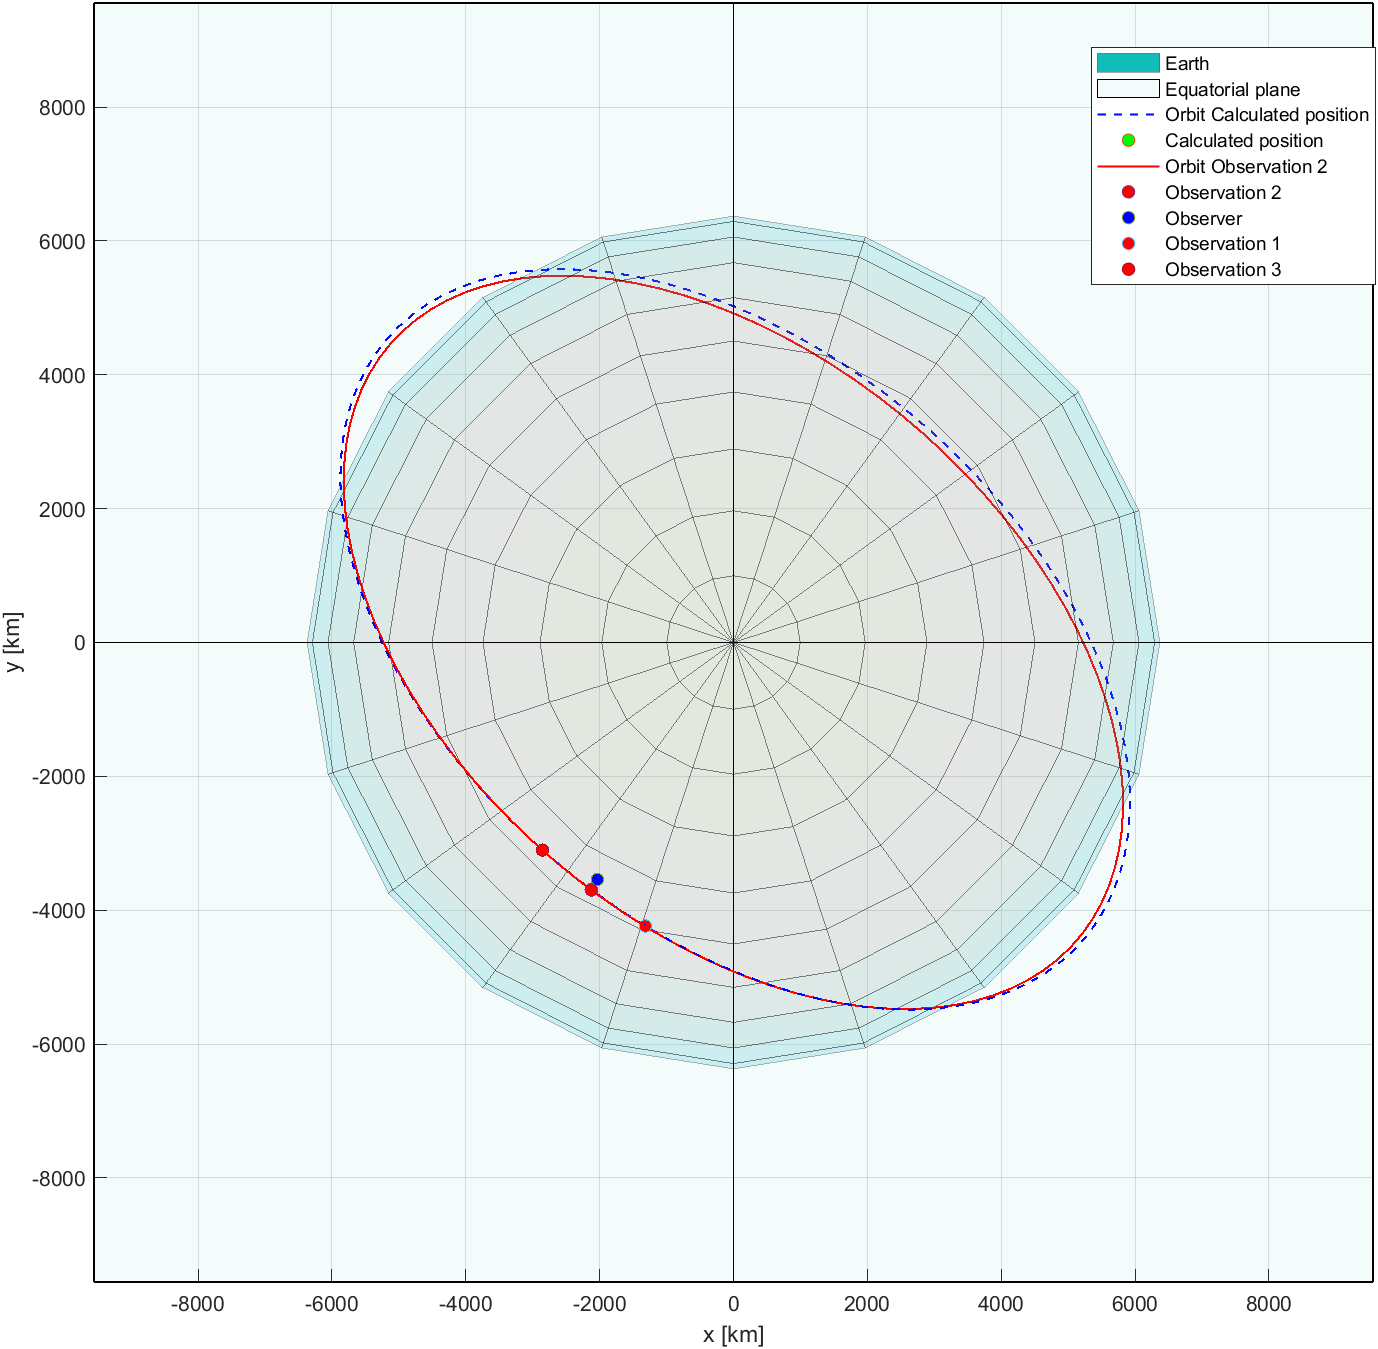
\includegraphics[width=\textwidth]{tex/img/StellariumFigure_rownikowa.png}
    \caption{Obserwacja na podstawie symulatora nieba - rzut na płaszczyznę równikową}
    \label{fig:Stellarium-2}
    \end{figure}
\FloatBarrier